%###############################################################################
%# N1 - Manual - Instruction set                                               #
%###############################################################################
%#    Copyright 2018 Dirk Heisswolf                                            #
%#    This file is part of the N1 project.                                     #
%#                                                                             #
%#    N1 is free software: you can redistribute it and/or modify               #
%#    it under the terms of the GNU General Public License as published by     #
%#    the Free Software Foundation, either version 3 of the License, or        #
%#    (at your option) any later version.                                      #
%#                                                                             #
%#    N1 is distributed in the hope that it will be useful,                    #
%#    but WITHOUT ANY WARRANTY; without even the implied warranty of           #
%#    MERCHANTABILITY or FITNESS FOR A PARTICULAR PURPOSE.  See the            #
%#    GNU General Public License for more details.                             #
%#                                                                             #
%#    You should have received a copy of the GNU General Public License        #
%#    along with N1.  If not, see <http://www.gnu.org/licenses/>.              #
%###############################################################################
%# Version History:                                                            #
%#   November 26, 2018                                                         #
%#      - Initial release                                                      #
%###############################################################################


\section{Instruction Set}
\label{opcodes}

The intent of the N1's instruction set is to map most of the essential Forth words
to single cycle instructions. \figref{opcodes:encoding} illustrates the basic structure
of the instructuion encoding.

\begin{figure}[!h]
  %\begin{center}
  \makebox[\textwidth][c]{
    \scalebox{0.75} {
      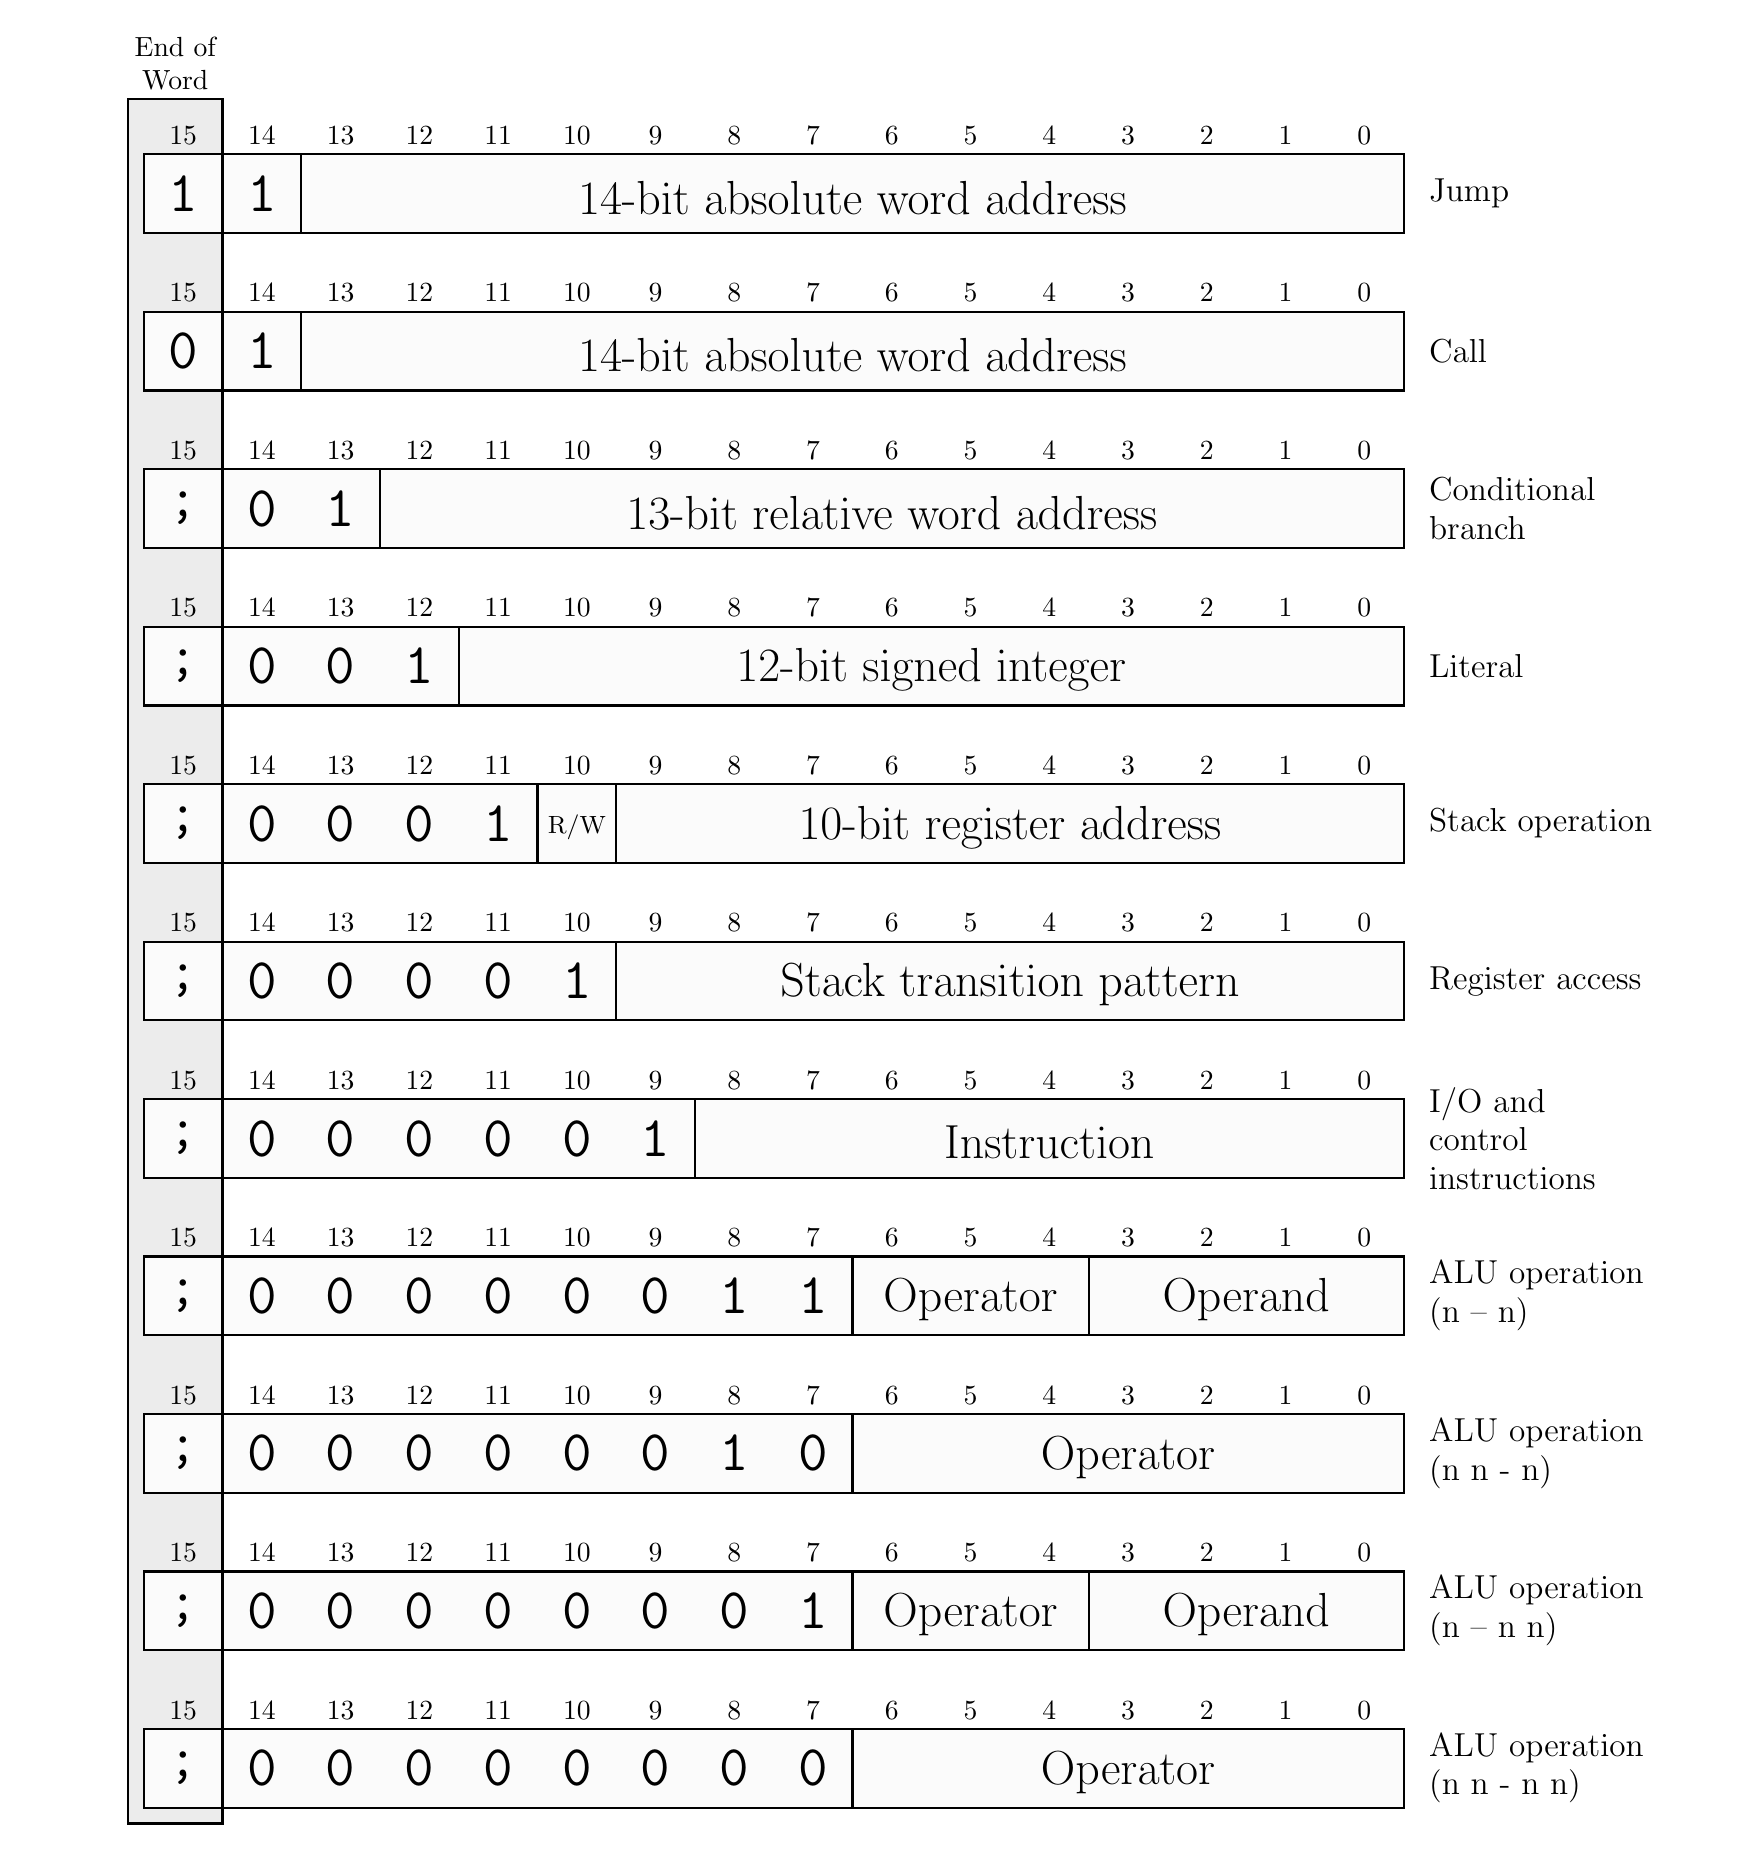
\begin{tikzpicture}
      
        %Instruction
        \newsavebox{\instruction}
        \savebox{\instruction}{
          \draw [thick, fill=gray!3] (0,0) rectangle (16,1);
          \draw [thick, fill=gray!3] (0,0) rectangle (1,1);
          \node [above] at (0.5,1)  {15};
          \node [above] at (1.5,1)  {14};
          \node [above] at (2.5,1)  {13};
          \node [above] at (3.5,1)  {12};
          \node [above] at (4.5,1)  {11};
          \node [above] at (5.5,1)  {10};
          \node [above] at (6.5,1)  {9};
          \node [above] at (7.5,1)  {8};
          \node [above] at (8.5,1)  {7};
          \node [above] at (9.5,1)  {6};
          \node [above] at (10.5,1) {5};
          \node [above] at (11.5,1) {4};
          \node [above] at (12.5,1) {3};
          \node [above] at (13.5,1) {2};
          \node [above] at (14.5,1) {1};
          \node [above] at (15.5,1) {0};
        };

        %Return bit
        \draw [thick, fill=gray!15] (0.8,0.3) rectangle (2,22.2);
        \node [above] at (1.4,22.2) {
          \begin{minipage}[c]{10em}
            \begin{center}
              End of\\
              Word
            \end{center}
          \end{minipage}};
      
        %Jump
        \node at (1,20.5) {\usebox{\instruction}};
        \node         at (1.5,21)     {\huge{\texttt{1}}};
        \draw [thick] (2,20.5) rectangle (3,21.5);
        \node         at (2.5,21)     {\huge{\texttt{1}}};
        \node         at (10,20.95)   {\LARGE{14-bit absolute word address}};
        \node [right] at (17.2,21)    {\large{Jump}};
     
        %Call
        \node at (1,18.5) {\usebox{\instruction}};
        \node         at (1.5,19)     {\huge{\texttt{0}}};
        \draw [thick] (2,18.5) rectangle (3,19.5);
        \node         at (2.5,19)     {\huge{\texttt{1}}};
        \node         at (10,18.95)   {\LARGE{14-bit absolute word address}};
        \node [right] at (17.2,19)    {\large{Call}};
       
        %Conditional Branch
        \node at (1,16.5) {\usebox{\instruction}};
        \node         at (1.5,17)     {\huge{\texttt{;}}};
        \draw [thick] (2,16.5) rectangle (4,17.5); 
        \node         at (2.5,17)     {\huge{\texttt{0}}};
        \node         at (3.5,17)     {\huge{\texttt{1}}};
        \node         at (10.5,16.95) {\LARGE{13-bit relative word address}};
        \node [right] at (17.2,17) {
          \begin{minipage}[l]{10em}
            \large{
              Conditional \\
              branch
            }
        \end{minipage}};
        
        %Literal 
        \node at (1,14.5) {\usebox{\instruction}};
        \node         at (1.5,15)     {\huge{\texttt{;}}};
        \draw [thick] (2,14.5) rectangle (5,15.5); 
        \node         at (2.5,15)     {\huge{\texttt{0}}};
        \node         at (3.5,15)     {\huge{\texttt{0}}};
        \node         at (4.5,15)     {\huge{\texttt{1}}};
        \node         at (11,14.95)   {\LARGE{12-bit signed integer}};
        \node [right] at (17.2,15)    {\large{Literal}};

        %Register access
        \node at (1,12.5) {\usebox{\instruction}};
        \node         at (1.5,13)     {\huge{\texttt{;}}};
        \draw [thick] (2,12.5) rectangle (6,13.5); 
        \draw [thick] (6,12.5) rectangle (7,13.5); 
        \node         at (2.5,13)     {\huge{\texttt{0}}};
        \node         at (3.5,13)     {\huge{\texttt{0}}};
        \node         at (4.5,13)     {\huge{\texttt{0}}};
        \node         at (5.5,13)     {\huge{\texttt{1}}};   
        \node         at (6.5,12.95)  {\small{R/\textoverline{W}}};   
        \node         at (12,12.95)   {\LARGE{10-bit register address}};
        \node [right] at (17.2,13)    {\large{Stack operation}};
        
        %Stack operation 
        \node at (1,10.5) {\usebox{\instruction}};
        \node         at (1.5,11)     {\huge{\texttt{;}}};
        \draw [thick] (2,10.5) rectangle (7,11.5); 
        \node         at (2.5,11)     {\huge{\texttt{0}}};
        \node         at (3.5,11)     {\huge{\texttt{0}}};
        \node         at (4.5,11)     {\huge{\texttt{0}}};
        \node         at (5.5,11)     {\huge{\texttt{0}}};   
        \node         at (6.5,11)     {\huge{\texttt{1}}};   
        \node         at (12,10.95)   {\LARGE{Stack transition pattern}};
        \node [right] at (17.2,11)    {\large{Register access}};

        %Control Instructions
        \node at (1,8.5) {\usebox{\instruction}};
        \node         at (1.5,9)       {\huge{\texttt{;}}};
        \draw [thick] (2,8.5) rectangle (8,9.5); 
        \node         at (2.5,9)       {\huge{\texttt{0}}};
        \node         at (3.5,9)       {\huge{\texttt{0}}};
        \node         at (4.5,9)       {\huge{\texttt{0}}};
        \node         at (5.5,9)       {\huge{\texttt{0}}};   
        \node         at (6.5,9)       {\huge{\texttt{0}}};   
        \node         at (7.5,9)       {\huge{\texttt{1}}};   
        \node         at (12.5,8.95)   {\LARGE{Instruction}};
        \node [right] at (17.2,9) {
          \begin{minipage}[l]{10em}
            \large{
              I/O and \\
              control \\
              instructions
            }
        \end{minipage}};
            
        %ALU operation (n -- n) 
        \node at (1,6.5) {\usebox{\instruction}};
        \node         at (1.5,7)      {\huge{\texttt{;}}};
        \draw [thick] (2,6.5) rectangle (10,7.5); 
        \draw [thick] (10,6.5) rectangle (13,7.5); 
        \node         at (2.5,7)      {\huge{\texttt{0}}};
        \node         at (3.5,7)      {\huge{\texttt{0}}};
        \node         at (4.5,7)      {\huge{\texttt{0}}};
        \node         at (5.5,7)      {\huge{\texttt{0}}};   
        \node         at (6.5,7)      {\huge{\texttt{0}}};   
        \node         at (7.5,7)      {\huge{\texttt{0}}};   
        \node         at (8.5,7)      {\huge{\texttt{1}}};   
        \node         at (9.5,7)      {\huge{\texttt{1}}};   
        \node         at (11.5,6.95)  {\LARGE{Operator}};
        \node         at (15,6.95)    {\LARGE{Operand}};
        \node [right] at (17.2,7) {
          \begin{minipage}[l]{10em}
            \large{
              ALU operation \\
              (n -- n)
            }
        \end{minipage}};
               
        %ALU operation (n n -- n) 
        \node at (1,4.5) {\usebox{\instruction}};
        \node         at (1.5,5)      {\huge{\texttt{;}}};
        \draw [thick] (2,4.5) rectangle (10,5.5); 
        \node         at (2.5,5)      {\huge{\texttt{0}}};
        \node         at (3.5,5)      {\huge{\texttt{0}}};
        \node         at (4.5,5)      {\huge{\texttt{0}}};
        \node         at (5.5,5)      {\huge{\texttt{0}}};   
        \node         at (6.5,5)      {\huge{\texttt{0}}};   
        \node         at (7.5,5)      {\huge{\texttt{0}}};   
        \node         at (8.5,5)      {\huge{\texttt{1}}};   
        \node         at (9.5,5)      {\huge{\texttt{0}}};   
        \node         at (13.5,4.95)  {\LARGE{Operator}};
        \node [right] at (17.2,5) {
          \begin{minipage}[l]{10em}
            \large{
              ALU operation \\
              (n n - n)
            }
        \end{minipage}};
            
        %ALU operation (n -- n n)
        \node at (1,2.5) {\usebox{\instruction}};
        \node         at (1.5,3)      {\huge{\texttt{;}}};
        \draw [thick] (2,2.5) rectangle (10,3.5); 
        \draw [thick] (10,2.5) rectangle (13,3.5); 
        \node         at (2.5,3)      {\huge{\texttt{0}}};
        \node         at (3.5,3)      {\huge{\texttt{0}}};
        \node         at (4.5,3)      {\huge{\texttt{0}}};
        \node         at (5.5,3)      {\huge{\texttt{0}}};   
        \node         at (6.5,3)      {\huge{\texttt{0}}};   
        \node         at (7.5,3)      {\huge{\texttt{0}}};   
        \node         at (8.5,3)      {\huge{\texttt{0}}};   
        \node         at (9.5,3)      {\huge{\texttt{1}}};   
        \node         at (11.5,2.95)  {\LARGE{Operator}};
        \node         at (15,2.95)    {\LARGE{Operand}};
        \node [right] at (17.2,3)   {
          \begin{minipage}[l]{10em}
            \large{
              ALU operation \\
              (n -- n n)
            }
        \end{minipage}};
               
        %ALU operation (n n -- n n)
        \node at (1,0.5) {\usebox{\instruction}};
        \node         at (1.5,1)      {\huge{\texttt{;}}};
        \draw [thick] (2,0.5) rectangle (10,1.5); 
        \node         at (2.5,1)      {\huge{\texttt{0}}};
        \node         at (3.5,1)      {\huge{\texttt{0}}};
        \node         at (4.5,1)      {\huge{\texttt{0}}};
        \node         at (5.5,1)      {\huge{\texttt{0}}};   
        \node         at (6.5,1)      {\huge{\texttt{0}}};   
        \node         at (7.5,1)      {\huge{\texttt{0}}};   
        \node         at (8.5,1)      {\huge{\texttt{0}}};   
        \node         at (9.5,1)      {\huge{\texttt{0}}};   
        \node         at (13.5,0.95)  {\LARGE{Operator}};
        \node [right] at (17.2,1) {
          \begin{minipage}[l]{10em}
            \large{
              ALU operation \\
              (n n - n n)
            }
        \end{minipage}};

      \end{tikzpicture}
    }
  }
  \caption{Instruction encoding}
  \label{opcodes:encoding}
  %\end{center}
\end{figure}

\subsection{Jump Instructions}
\label{opcodes:jump}

\Gls{jump} instructions transfer the program flow to any \gls{word}
location within the supported 32KB program space. \Gls{jump} instructions
use absoluteaddresses. 

\subsection{Call Instructions}
\label{opcodes:call}

\Gls{call} instructions temporarily transfer the program flow to any \gls{word}
location within the
supported 32KB program space, while pushing a return address onto
the return stack \gls{call} instructions use absolute addresses. 

\subsection{Return from a Call (\texttt{;})}
\label{opcodes:rtc}

Rather than  providing a dedicated instruction to end the execution of 
word in Forth and to return the program flow to its caller, the N1 allows
to perform this operation in parallel to the execution of any of its
instructions. Each \gls{opcode} contains a bit (bit 15) to indicate, that the
current instruction in the last operation in the current word. If this bit
is set, the program flow will resume at the calling word as soon as the
operationis performed.

As shown in \figref{opcodes:encoding}, bit 15 is also used to distinguish jump
and call. Considering that the last call in a word definition can be optimized
to a jump to the first instruction of the called word, bit 15 can ber regarded
as termination bit for these instructions as well.

For a Forth compiler, this means that the semi-colon (\texttt{\gls{semicolon}})
always translates to setting bit 15 of the last instruction.

\subsection{Conditional Branches}
\label{opcodes:branch}

Conditional \glspl{branch} invoke a change of program flow if the top of the
\gls{ps} is not zero. Branches are relative to the location of the
following instruction and range from 4095 \gls{word}
locations forward to 4096 \gls{word}
locations backward. A relative \gls{branch}
address of zero points to the subsequent instruction of the current one.

Conditional branches use relative addressing to simplify code reallocation in support
of inlining.

\subsection{Literals}
\label{opcodes:literal}

Signed integer \glspl{literal} of 12-bit length can be pushed onto the \gls{ps} within
a single instruction. For larger integers a supplemental TBD \gls{call} is required.

\subsection{Register Accesses}
\label{opcodes:regacc}


\subsection{Stack Operation}
\label{opcodes:stack}

The N1's stack instruction aims at efficiently implementing the essential stack operations
in \Gls{forth} only using the data pathes which needed for the stack's push and pull
operations.

The opcode of the stack instruction contains a 10-bit wide field to specify a transition pattern of the upper elements of the \gls{ps} and the \gls{rs}.




\subsection{I/O and Control Instructions}
\label{opcodes:ioctrl}
\Gls{byte}

\subsection{ALU operations}
\label{opcodes:ioctrl}
